\documentclass[a4,12pt]{article}

\usepackage[utf8]{inputenc}
\usepackage[spanish]{babel}
\usepackage[margin=1.5cm]{geometry}
\usepackage{graphicx}
\usepackage{color}
\usepackage{import}
\usepackage{float }



\usepackage{hyperref}

\parindent 0em

%\usepackage{times}
\renewcommand{\familydefault}{\sfdefault}

\title{Breve introducción a GNU OCTAVE}
\author{Youssef Said Khloufi}
%\date{}

\begin{document}

\maketitle
\bigskip
\bigskip
\bigskip
\begin{figure}[H]
  \centering
    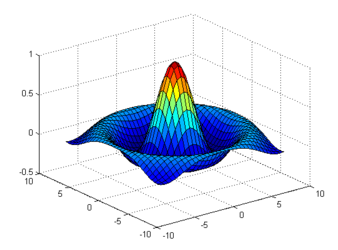
\includegraphics{graficos/octave}
\end{figure}
\newpage

\maketitle

\begin{abstract}
Este documento explica de manera muy breve los fundamentos y características principales del software libre GNU Octave.

\end{abstract}

\tableofcontents
\newpage

\section{Introducción}

OCTAVE : Lenguaje numérico de programación de libre acceso.

\subsection{Características principales de OCTAVE}

- Programa específico de Cálculo Numérico.\\
• Sólo opera con Números.\\
• Se puede considerar como una calculadora programable muy potente.\\
\medskip\\
-Programa muy popular entre estudiantes, ingenieros, técnicos e investigadores debido a sus características:\\
• Programa de libre acceso.\\
• Programa interactivo.\\
• Capacidades Gráficas sencillas.\\
• Posee gran cantidad de Funciones de todos los tipos.\\
• Lenguaje de programación de alto nivel similar a Fortran, C, Pascal o Basic, pero más  fácil de aprender.\\
Su lenguaje de programación es igual al de MATLAB.

\subsection{Acceso a OCTAVE desde el entorno Unix}

• Ejecutar la instrucción octave desde cualquier ventana de consola (tiene que estar instalado)\\
• Aparece la siguiente ventana del octave:\\
\begin{verbatim}
    octave:1>
\end{verbatim}

\subsection{Accesos a OCTAVE desde windows}

• Hacer doble click sobre el icono de OCTAVE.\\
• Al igual que en el entorno Unix , aparece la ventana del octave (consola).

\subsection{Algunas instrucciones de utilidad }

-\textbf{pwd:} nos dice en que directorio nos encontramos.\\
-\textbf{ls:} nos da una lista de los ficheros y los directorios\\
-\textbf{cd:} nombre nos permite cambiar al directorio nombre.

\subsection{Operaciones básicas.}

\begin{verbatim}
    + adición
    - sustracción
    * multiplicación
    ^ potenciación
    \ división izquierda
    / división derecha
\end{verbatim}

\begin{verbatim}
    exp   log   exponencial y logaritmo neperiano
    sin   cos   seno y coseno
    abs   sqrt  valor absoluto y raíz cuadrada
    round floor ceil funciones que redondean
\end{verbatim}

Ejemplos:

\begin{verbatim}
    > 2 + 3         > 2 * 2
    ans = 5          ans = 4

    > sin(pi/6)     > 2/6
    ans = 0.50000    ans =0.33333

    > log(5^3)      > round(4.5)
    ans = 4.8283     ans = 5

    > ceil(4.5)     > floor(4.5)
    ans = 5          ans = 4
\end{verbatim}

• Observe que: los () se reservan sólo para escribir el argumento de las funciones.

\subsection{Ayudas y normas generales del OCTAVE}

• El comando help nos proporciona información sobre las funciones del OCTAVE:\\
\begin{verbatim}
    > help round   % redondea al entero mas cercano
    > help floor   % redondea por defecto
    > help ceil    % redondea por exceso
\end{verbatim}
• Las flechas: arriba y abajo permiten recuperar comandos anteriores.\\
• Las flechas: izquierda y derecha permiten movernos a lo largo de una línea de instrucciones y corregirla.\\
• OCTAVE distingue entre mayúsculas y minúsculas:\\
\begin{verbatim}
    > ceil(2.3)
    ans = 3
\end{verbatim}
\textbf{NO} es lo mismo que:\\
\begin{verbatim}
    > Ceil(2.3)
    error: ‘Ceil’ undefined near line 22 column 1
\end{verbatim}
• Podemos asignar variables con determinados nombres a las expresiones numéricas (números,constantes).\\
\begin{verbatim}
    > m = 9.11e-31; q = -1.6e-19;
    > r = abs(q)/m
    r = 1.7563e+11
    > 3e+8
    ans = 300000000
    > m*(ans^2)
    ans = 8.1990e-014
\end{verbatim}
• Los nombres de estas variables pueden formarse utilizando letras,dígitos, etc.\\
• Las variables se pueden borrar con el comando \textbf{clear} nombre.\\
• Asignación por defecto: si a una expresión numérica no le asignamos un nombre, OCTAVE crea la variable ans.\\
• El comando \textbf{who} nos permite conocer los nombres de las variables asignadas. Ejecute \textbf{who}

\section{Vectores}

\begin{verbatim}
    vector: conjunto de números a1, a2, ..., an
\end{verbatim}
\begin{figure}[H]
  \centering
    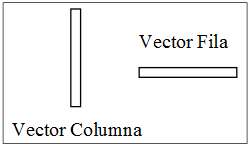
\includegraphics[width=0.5\textwidth]{graficos/imagen1}
\end{figure}

\subsection{Vectores fila y vectores columnas}

• Para definir vectores utilizamos los corchetes [ ].\\
• Los elementos de una fila se separan mediante espacios en blanco o comas .\\
• Los elementos de una columna se separan por puntos y comas o por nuevas líneas.\\
\begin{verbatim}
    > A=[ 1 2 3 4 5 6 7 8 9]; % vector fila
    > vecf=[1,2,3,4,5,6,7,8,9]; % vector fila
    > B=[ 1
    > 2
    > 3
    > 4 ]; % vector columna
    > vecc=[1;2;3;4]; % vector columna
\end{verbatim}
• El \% se utiliza en OCTAVE para escribir comentarios.

\subsection{Utilización de los dos puntos}

• 1er elemento del vector : incremento : último elemento.\\
• 1er elemento del vector : último elemento y OCTAVE toma toma el incremento = 1.\\
\begin{verbatim}
    > A=1:2:5
    A = 1 3 5
    > B=[5:-1:3]’
    B =
      5
      4
      3
    > x = [0:0.1:2*pi]’;
    > y = sin(x);
    > [x y]
\end{verbatim}

\subsection{Funciones sobre los vectores}

• \textbf{length} : calcula el número de elementos de un vector (longitud de un vector). Su argumento es el propio vector.

• \textbf{sin} : si el argumento de la función seno es un vector entonces, esta función calcula el seno de cada elemento del vector. El argumento de las funciones trigonométricas debe de estar expresado en radianes.
\begin{verbatim}
    > v=[0.1:0.1:0.6]
    v = 0.1000 0.2000 0.3000 0.4000 0.5000 0.6000

    > sin(v)
    ans = 0.0998 0.1987 0.2955 0.3894 0.4794 0.5646

    > length(v)
    ans = 6
\end{verbatim}

\subsection{Operaciones vectoriales y Operaciones puntuales}

\medskip
\begin{center}
\begin{tabular}{|c|c|} \hline
\textbf{Operaciones}   &  \textbf{Operaciones puntuales} \\ \hline
+     suma & +     suma \\  \hline
-     resta & -     resta \\ \hline
*     multiplicacion & .*     multiplicacion \\  \hline
/     division derecha & ./     division derecha \\ \hline
ˆ     potenciacio & .ˆ     potenciacio \\ \hline
\end{tabular}
\end{center}

\textbf{• Las operaciones puntuales} se utilizan para realizar operaciones entre vectores y matrices. Por ejemplo si queremos multiplicar cada elemento del vector x por el correspondiente elemento del vector y, siendo x = (1,-2,4,2) e y = (3,-5,4,0), escribimos.
\begin{verbatim}
    % definimos los elementos de los vectores
    > x = [1 -2 4 2]; y = [3 -5 4 0];
     % utilizamos la multiplicaci\’on puntual
    > x.*y
    ans=
      3 10 16 0
\end{verbatim}

\section{Editor del OCTAVE. Programación}

Para editar un programa nuevo, desde la misma ventana del OCTAVE , escribir el comando \textbf{edit}.

\subsection{Tipos de m-files}

• Archivos de instrucciones (estos archivos se ejecutan directamente desde la ventana del OCTAVE ). prac.m
\begin{verbatim}
    % Este es el programa prac.m y se guardan los valores
    % de la intensidad (I) y del voltage (V)
    I=[0.01;0.02;0.03;0.036;0.032;0.028;0.024;0.018;0.012;0.008];V=[3.04;6.41;
    9.84;11.73;10.61;9.02;7.65;5.71;3.79;2.55];
\end{verbatim}

Para ejecutarlo y realizar operaciones con las variables guardadas:
\begin{verbatim}
    > clear
    > help prac
    % En el programa prac.m se guardan los valores
    % de la intensidad (I) y el voltage (V)
    > prac         % ejecutamos el programa
    > plot(I,V)    % dibuja V(I)
\end{verbatim}

\textbf{Observaciones importantes:}\\
• Los ficheros deben ser escritos en ASCII . La extensión del programa es \textbf{.m}\\
• El programa debe de ejecutarse desde el directorio donde se encuentre.

\section{Secuencias}

Una forma sencilla de producir una secuencia de números es utilizando la notación n:m
donde n es el número inicial y m el final

\begin{verbatim}
	octave:2> 1:10 ans =

	1	2	3	4	5	6	7	8	9	10
\end{verbatim}

También podemos usar la notación p:q:r para crear una secuencia que inicia en p, finaliza en r con intervalos de q. En el siguiente caso almacenaremos en una variable b una secuencia partiendo de cero y finalizando en diez, con un intervalo de dos entre cada número.

\begin{verbatim}
	octave:3> b=0:2:10 b =

	0	2	4	6	8	10
\end{verbatim}

Tenemos	otras	dos	funciones	que	nos	permiten	crear	vectores	de	elementos secuenciales,  estos  son  linspace y  logspace,  el  primero  separa  los  números uniformemente y el segundo lo hace logarítmicamente.

\begin{verbatim}
	octave:39> linspace(1,4,6)
	ans =

	1.0000	1.6000	2.2000	2.8000	3.4000	4.0000
\end{verbatim}

\section{Sistema de ecuaciones}

Para la resolución de sistemas de ecuaciones del tipo Ax = b utilizamos la notación a\b, por ejemplo, para calcular el siguiente sistema de ecuaciones de primer grado con dos incógnitas
\begin{verbatim}
    6·x - 7·y = 5
    8·x - 9·y = 7
\end{verbatim}
haremos lo siguiente: guardaremos los elementos \textbf{x} e \textbf{y} en una matriz \textbf{a} y la igualdad en un vector \textbf{b}, para finalmente ejecutar el comando \textbf{a\textbackslash b}.
\begin{verbatim}
    octave:4> a=[6, -7;8,-9]
    a =

    6	-7
    8	-9
    
    octave:5> b=[5;7]
    b =

    5
    7

    octave:6> a\b ans =

    2
    1
\end{verbatim}

\section{Funciones definidas por el usuario}

En Octave podemos crear nuestras propias funciones, podemos escribirlas directamente desde la línea de comandos o ejecutarlas desde un archivo externo.

Las funciones que creamos desde la línea de comandos deben cumplir con el siguiente formato:
\begin{verbatim}
    function variable_salida = nombre_funcion (argumentos_entrada)
      cuerpo _funcion 
    endfunction
\end{verbatim}
En caso de devolver varias variables, éstas deben estar encerradas entre corchetes
“[ ]”:
\begin{verbatim}
    function [salida1,salida2] = nombre_funcion (argumentos_entrada)
      cuerpo _funcion 
    endfunction
\end{verbatim}
Por ejemplo, crearemos una función que calcula el seno(x) en grados:
\begin{verbatim}
    octave:1> function s = sind(x)
    > %SIND(X) Calcula seno(x) en grados
    > s = sin(x*pi/180);
    > endfunction
\end{verbatim}
Y ejecutamos,
\begin{verbatim}
    octave:2> sind(45)
    ans = 0.70711

    octave:3> sind(90)
    ans = 1
\end{verbatim}
Para que Octave ejecute un archivo éste debe tener extensión \textbf{.m} y debe encontrarse en el directorio desde donde estemos ejecutando Octave. También podemos agregar rutas adicionales con el comando  addpath('ruta'), donde ruta es el camino al directorio que contiene los scripts. Para borrar la ruta usamos rmpath('ruta').
Ejemplo: Suma de los elementos que integran una matriz, \textbf{sumaelementos.m}
\begin{verbatim}
    M=[round(rand(3,3)*100)]  % creamos una matriz aleatoria de 3x3
    [f,c]=size(M);            % f #filas; c #columnas
    s=0;                      % inicializamos s=0 (suma inicial)
    for i = 1:f               % recorre filas
      for j=1:c               % recorre columnas (en cada fila)
        s=s+M(i,j);           % suma cada elemento a s
      end
    end
    s                         % muestra la suma final
\end{verbatim}
Para ejecutarlo escribiremos el nombre del archivo en la línea de comandos, deberá aparecer lo siguiente,
\begin{verbatim}
    octave:1> sumaelementos
    M =
    96 77 77
    36 29 58
    19 63 71
    s = 526 
\end{verbatim}
Para crear programas donde el usuario  debe introducir datos utilizamos el comando \textbf{input} dentro del archivo.

Ejemplo: Función que convierte kilos en libras, kilo2libra.m
\begin{verbatim}
    %*******************************************************************
    % kilo2libra.m
    % Programa que permite convertir un valor en kilos a libras.
    %*******************************************************************
    disp('\nPrograma de conversion de kilos a libras\n'); kilo = input(
    'Introduzca el peso en kilogramos: '); libra=kilo*2.20462262185;
    fprintf('\n%g kilogramos son %f libras.\n', kilo, libra);
    %*******************************************************************
\end{verbatim}
Haremos la conversión de 40 kilogramos en libras,
\begin{verbatim}
    octave:2> kilo2libra

    Programa de conversion de kilos a libras

    Introduzca el peso en kilogramos: 40

    40 kilos son 88.184905 libras.
\end{verbatim}

\section{Gráficos}

\subsection{Gráficos en 2 dimensiones}

• Dada un conjunto de n puntos ( x i , y i), i = 1, 2, ..., n, definidos previamente en los vectores x e y del OCTAVE ; la instrucción \textbf{plot(x,y)} nos dibuja los pares de puntos (x i , y i) unidos por líneas. Ejecuta \textbf{help plot}.

• \textbf{plot(x,y,’cts’)} , donde c es el color de las líneas, \textbf{t} el tipo de líneas y s el símbolo que usa OCTAVE para dibujar los puntos.
\begin{center}
\begin{tabular}{|c|c|c|} \hline
\textbf{Color} &  \textbf{Tipos de lineas} & \textbf{Simbolos} \\ \hline
y yellow & . point & - solid \\ \hline
m magenta & o circle & : dotted \\ \hline
c cyan & x x-mark & -. dashdot \\ \hline
r rojo & + plus & – dashed \\ \hline
g green & * star &  \\ \hline
b blue & s square &  \\ \hline
w white & d diamond &  \\ \hline 
k black &  &  \\ \hline 
\end{tabular}
\end{center}

\textbf{Ejemplo:} Gráficos múltiples. Varias curvas en el mismo gráfico.\\
\begin{verbatim}
    > x=0:.01:2*pi;
    > y1=sin(x);y2=sin(2*x);y3=sin(3*x);
    > plot(x,y1,x,y2,’--’,x,y3,’.’)
\end{verbatim}

\begin{figure}[H]
  \centering
    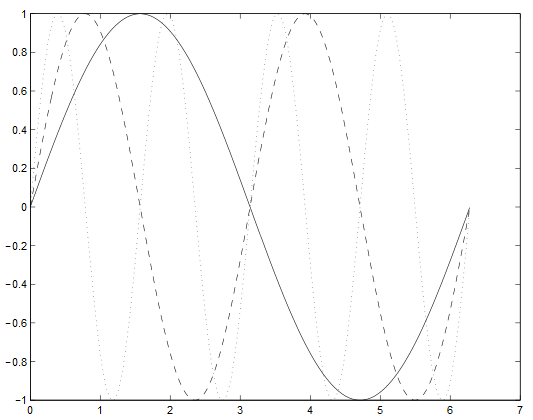
\includegraphics[width=0.5\textwidth]{graficos/imagen7}
\end{figure}

• Utilización del \textbf{hold on} , \textbf{hold off} y el \textbf{clf}\\
\begin{verbatim}
    > clf
    > x=0:.01:2*pi;
    > y1=sin(x);y2=sin(2*x);y3=sin(3*x);
    > plot(x,y1)
    > hold on
    > plot(x,y2,’--’); plot(x,y3,’.’)
    > hold off
\end{verbatim}
\textbf{Funciones gráficas}\\
\smallskip
• clf borra la pantalla gráfica.
• hold on permite añadir al último gráfico una nueva figura.
• hold off desactiva el hold on.
• axis([ xmin,xmax,ymin,ymax ]) escala la ventana gráfica.
• grid dibuja una retícula cuadrada.
• x label(’ nombre del eje x ’) , y label(’ nombre eje y’),title(’título’).

\subsection{Gráficos en 3 dimensiones}

Para producir gráficos en 3D disponemos de varias opciones, la mas simple es usar el comando  plot3(x,y,z) donde cada argumento es tomado para convertirse en los vértices del gráfico tridimensional.

Si todos los argumentos son vectores de la misma longitud se dibujará una única línea continua. En caso de todos los argumento sean matrices cada una de las columnas de las matrices serán tratada como líneas separadas.

En caso de que sólo se le pasen dos argumentos en lugar de tres, plot3(x,c), el segundo argumento 'c' debe ser un número complejo, así, las partes reales e imaginarias de éste son usadas como las coordenadas y e z respectivamente.

Si sólo se le pasa un argumento, plot3(c), las partes reales e imaginarias de los argumentos son usados como los valores y y z, y se trazan frente su índice.

El comando plot3 también acepta los argumentos que permiten modificar el formato de presentación de la gráfica descritos en la sección de gráficas bidimensionales.

Ejemplo:\\
\begin{verbatim}
	  octave:51> z = [0:0.05:5];
    octave:52> plot3(z, exp(2i*pi*z), "3;sinusoidal compleja;")
\end{verbatim}
\begin{figure}[H]
  \centering
    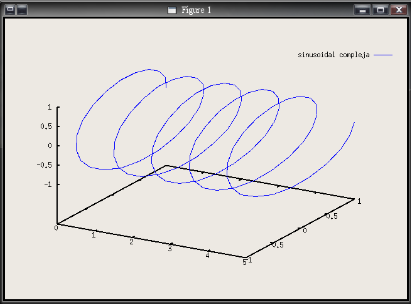
\includegraphics[width=0.5\textwidth]{graficos/imagen4}
  \caption{Gráfica de una sinusoidal compleja con 'plot3()'}
\end{figure}

El comando mesh(x,y,z) hace una representación tridimensional dado dos vectores x e y,  y  una  matriz  bidimensional  z.  Generalmente  se  usa  el  comando  meshgrid para generar los datos que usará mesh para para representar los ejes x e y.

\textbf{Ejemplo:}
\begin{verbatim}
	octave:1> x=[-2:0.1:2];	% genera el vector
	octave:3> [xx,yy] = meshgrid(x,x);	% genera las matrices de ejes octave:4> 
	z=sin(xx.^2 – yy.^2);	% funcion z=sen(x^2 – y^2) octave:5> grid	% genera 
	una rejilla
	octave:6> mesh(x,x,z)	% crea el grafico
\end{verbatim}
\begin{figure}[H]
  \centering
    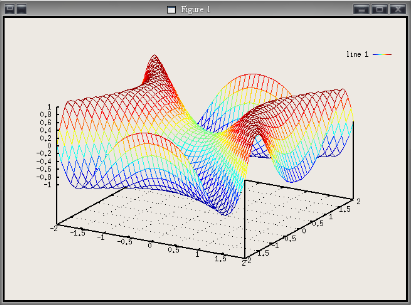
\includegraphics[width=0.5\textwidth]{graficos/imagen5}
  \caption{Generación de gráficos mediante 'mesh()'}
\end{figure}

La función contour(x,y,z) recibe los mismos argumentos que mesh() y dibuja las curvas de nivel de la superficie.

Vamos a generar las curvas de nivel del gráfico generado en el ejemplo anterior:

\begin{verbatim}
	octave:10> contour(x,x,z);
\end{verbatim}
\begin{figure}[H]
  \centering
    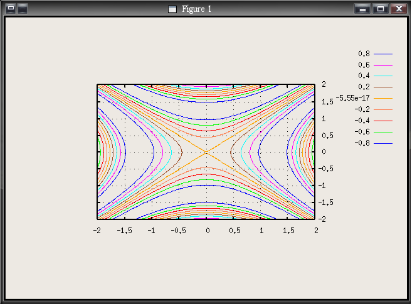
\includegraphics[width=0.5\textwidth]{graficos/imagen6}
  \caption{Curvas de nivel generadas por medio de 'contour()'}
\end{figure}

\section{Grabar y leer datos en ficheros. Impresión de las gráficas}

• La instrucción save fname. mat x y z graba las variables a b c en el fichero fname. mat ( archivos mat o MAT-files).\\
• La instrucción load fname. mat recupera las variables guardadas en el archivo fname. mat.\\
\smallskip
\textbf{Ejemplo:}\\
\begin{verbatim}
    > clear; clf
    > x = [0:pi/60:2*pi]; y = sin(x.^2);
    > save datos.mat x y
    > clear
    > who
    > load datos.mat
    > who
    > x
    > plot(x,y)
\end{verbatim}
• Para imprimir la figura en un archivo postscript utilizamos el comando \textbf{print -dps nfile.ps} . Por ejemplo, \textbf{print -dps fig.ps} crea el archivo postscript, fig.ps, de la figura que este en la ventana gráfica del OCTAVE.

\end{document}
